\section*{Series de Tiempo}

\subsection*{Introducción}
Muchos autores han escrito sobre las series de tiempo, pero es difícil agregar al tema o discutir las ideas del profesor Robert Hyndman, uno de los expertos más respetados en la comunidad de la estadística por su trabajo en las series de tiempo. Hyndman extiende la teoría a las series de tiempo como elementos de pronostico y su relación con la regresión lineal (Hyndman, R., 2014). Desde el punto de vista técnico, Hyndman es el creador de varias bibliotecas de funciones de pronostico utilizando series de tiempo y ARIMA en lenguaje R. Dentro de la bibliografía, Daroczi es quien agrega detalles sobre la detección temprana de valores atípicos que pueden dificultar – y mucho – el análisis (Daróczi, G., 2015). 

\subsection*{Introducción a las Series de Tiempo}
Las series de datos son muy útiles para pronosticar algo que cambia con el tiempo. Ejemplos de estas cantidades que varían con el tiempo incluyen acciones en la bolsa de valor, cifras de ventas, y otro tipo de información cuantitativa.

En forma general cualquier cosa que observamos secuencialmente en el tiempo es una serie de tiempos \cite{hyndman}. La literatura académica se concentra en series de tiempo que se observan en intervalos regulares de tiempo, aunque aquellas que se observan en intervalos irregulares también existen. 

En el pronóstico de series de tiempo, la idea principal es estimar cómo la secuencia de observaciones continuará en el futuro. El pronóstico de series de tiempo utiliza solamente información de la variable a ser pronosticada, y no hace intento alguno de descubrir cuales son los factores que motivan este comportamiento (en análisis de regresión diríamos que buscamos las variables de confusión). Por lo tanto el análisis de series de tiempo extrapola la tendencia secular y los patrones cíclicas, pero ignora todo otro tipo de información que puede afectar el movimiento de la variable estudiada, como pueden ser en la vida real efectos de la publicidad en el lanzamiento de un producto, la tasa de cambio en las ventas, o actividades de riesgo en el precio internacional de materias primas. 

Podemos ver un ejemplo de serie de tiempo si tomamos los valores de la TRM (la Tasa Representativa de Mercado, el nombre oficial de la tasa de cambio del dólar en Colombia) en la siguiente gráfica:\\

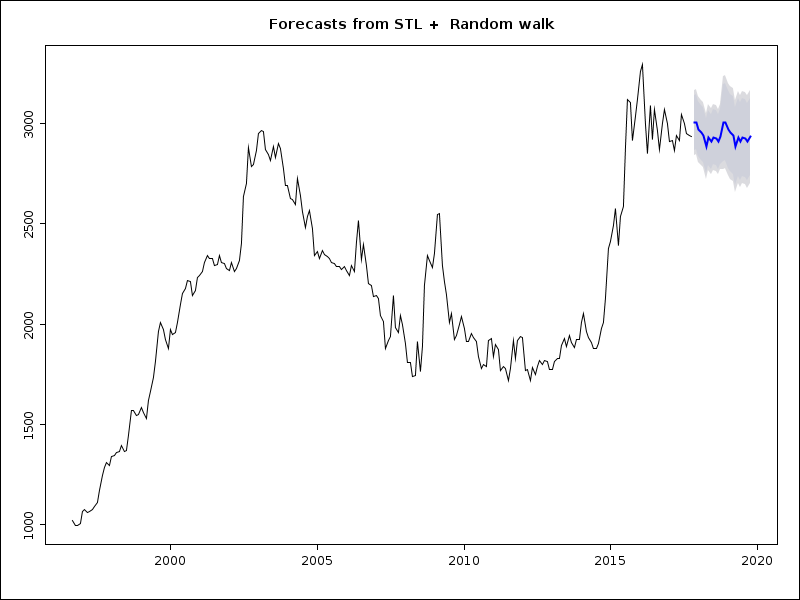
\includegraphics[width = 4 in]{timeSeries1.png}\\

La línea negra es la variación de la TRM a lo largo del tiempo (en este caso, desde el año 1980 hasta el 2017). La línea azul es el pronóstico del valor de la TRM según la función \texttt{forecast()} del lenguaje R. La zona gris comprenden el intervalo de confianza del pronóstico, la cual nos da una idea más real de como puede fluctuar el pronóstico dentro del mismo. 

\subsubsection*{Variables de Predicción en Series de Tiempo}
Es posible utilizar predictores en el pronóstico de series de tiempo. Un ejemplo utilizando el tema de investigación de este mismo trabajo es el pronóstico de la TRM, la cual estimamos es el resultado de varios factores:

\[ TRM = f(\textnormal{demanda dólar, tasa interés, turismo, error}) \]

La relación no es exacta, sino que siempre habrá factores por lo cuales el modelo no puede responder. Estas variaciones están previstas en el término error dentro del modelo. Este tipo de modelo se llama \emph{modelo explanatorio}. 


\subsection*{Pronóstico con Series de Tiempo}
Los pronósticos con series de tiempo utilizan solamente la información disponible de la variable que se propone pronosticar, sin hacer intento alguno por descubrir los factores adicionales que condicionan su comportamiento. Por lo tanto se extrapolan las tendencias y patrones temporales, pero se ignora toda la informacion adicional como pueden ser iniciativas de publicidad, actividad de la competencia, cambios en las condiciones económicas y otros \cite{hyndman}.

\subsection*{Patrones}
Las series de tiempo pueden descomponerse según su patrón o tendencia en tres elementos que las componen [Velazco, M., 2017]. A saber:

\begin{enumerate}
	\item Tendencia Secular: la tendencia secular o tendencia a largo plazo de una serie de tiempo es por lo común el resultado de factores a largo plazo. 
	\item Variación Estacional: Es el componente de la serie de tiempo que representa la variabilidad de los datos debido a la influencia de las estaciones.
	\item Variación Irregular: Esta variación se debe a factores a corto plazo, imprevisibles, y no recurrentes que afectan la serie de tiempo. 
\end{enumerate}

\subsection*{Auto Correlación}
De igual manera que una correlación mide la extensión de una relación linear entre dos variables, la autocorrelación mide la relación linear entre dos valores retrasados de series de tiempo \cite{hyndman}.

El valor de una autocorrelación para un \(r_{k}\) dado es:

\[ r_{k} = \frac{\sum_{t = k + 1}^T(y_{t} - \bar{y})(y_{t - k} - \bar{y})}{\sum_{t = 1}^T(y_{t} - \bar{y})^{2}} \]

donde \(T\) es el valor de período temporal de la serie de tiempo. 

El autor Daroczi agrega como metodología para la verificación de autocorrelación en un juego de datos (no solo una serie de tiempos, sino cualquier juego de datos espacial) el \emph{Indice I de Moran} \cite{daroczi}. Dicho índice esta dado por la formula:

\[ I = \frac{N}{W} 
	\frac{\sum{i}\sum{j}w_{ij}(x_{i} - \bar{x})(x_{j} - \bar{x})}{{\sum{i}(x_{i} - \bar{x})^2}} \]

\subsection*{Precisión del Pronostico}
Existen dos formas que se utilizan comúnmente para medir la precisión del pronóstico de series de tiempo. Ambas están basadas en el error absoluto o error cuadrático \cite{hyndman}.

\[Error Promedio Absoluto (MAE) = promedio(|e_{i}|)\]

\[ Error Promedio Cuadratico (RMSE) = \sqrt{promedio(e_{i}^2)}  \]

La tendencia al comparar precisión en un solo juego de datos es utilizar el MAE ya que es mas sencillo y simple de entender. 

\subsection*{Entrenamiento y Evaluación}
Al igual que la mayoría de los métodos de aprendizaje automatizado, las series de tiempo se suelen entrenar y evaluar con juegos alternos de muestra de datos. El tamaño de cada uno varía con el investigador, pero en serie de datos el sistema operativo tiende a ochenta por ciento de la muestra para entrenamiento y veinte por ciento para evaluación \cite{hyndman}.

\subsection*{Descomposición de Series de Tiempo}
La descomposición de las series de tiempo facilita el análisis y la investigación exploratoria de los datos. Una de las formas mas sencillas de lograr esto es la aplicación de promedios móviles, lo cual se facilita mucho en R con el uso de la función \texttt{decompose()} \cite{daroczi}.

La descomposición por promedios móviles toma la forma siguiente:

\[ s_{t} = \frac{1}{k} \sum_{n = 0}^{k - 1} x_{t - n}  \]

Muchas series de tiempo no son aditivas sino multiplicativas, y con el paso del tiempo incrementan la amplitud de las fluctuaciones. Para tales series, la biblioteca de R tiene la función \texttt{stl()} que aplica descomposicion a base del método Loess. La aplicacion del método Loess y la transformación de la función a una logarítmica tiene el efecto de replicarla como aditiva \cite{viswanathan}.

\subsection*{Suavizar Exponencialmente con Holt-Winters}
Es posible eliminar todos los efectos de estacionalidad en una serie de tiempo con la aplicacion del filtro Holt-Winters. Esto no solo resulta en una lectura mas clara de la tendencia secular de la serie, útil para pronósticos, sino que adicionalmente tiene el efecto de eliminar valores atípicos (outliers) en la misma \cite{daroczi}.

\subsection*{ARIMA}
Uno de los métodos mas populares para la descomposición de series de tiempo con periodos de doce meses es ARIMA, el cual fue desarrollado por el Buró de Censo de Estados Unidos \cite{hyndman}. El método esta basado en la descomposición tradicional, pero tiene la ventaja de mantener la tendencia secular en todos los puntos de datos, y de permitir que la tendencia estacional varíe de a poco con el tiempo. Es también un método muy robusto.

\subsection*{Dickey-Fuller} 
Un componente importante de las series de datos es la detección de si son o no auto-regresivas (lo que determina mucho de su poder predictivo). La fórmula para la detección de series auto-regresivas es el test Dickey-Fuller, y la mejor bibliografía es el artículo científico escrito por ambos profesores en la revista especializada Econometrica (Dickey, D., y Fuller, W., 1981). A pesar de ser un artículo contemporáneo, la teoría detrás de la prueba Dickey-Fuller nos permite descartar series de tiempo no-regresivas con poco poder de predicción. 
